\section{多体结构与实现}
\label{physics:section}

前文构造实现了共同单比特几何的调节。本节先确定测量态的多体纠缠，再考察测量酉的相位分解与 Clifford 层级。

\subsection{真正多体纠缠}
\label{physics:entanglement}
\label{physics:endpoints}

先直接证明：对每个 $n\ge5$ 和任意实参数 $t$，每个测量列均真正多体纠缠。记 $\psi(y)=\braket{y}{\psi_0(t)}$、$u=e^{it}$。逆向通过式~\eqref{core:phase-family} 的 CNOT 链得到 $w_j=y_j\oplus y_{j+1}$（$j<n$），并记 $w^{(b)}=(w_1,\ldots,w_{n-1},b)$。末位 Hadamard 门于是给出
\[
 \sqrt{2^{n+1}}\,\psi(y)
 =D_{n,t}(w^{(0)})+(-1)^{y_n}D_{n,t}(w^{(1)}).
\]
对 $y=1^n$，两个输入串为 $0^n$ 和 $e_n$，相位均为 $1$，故 $\psi(1^n)=0$。对单翻转邻居 $y=1^n\oplus e_j$，代入核~\eqref{core:kernel} 可知：当 $j=1,n$ 时，两个输入的重量为 $1,2$，且均有 $d_n=0$；当 $2\le j\le n-1$ 时，重量为 $2,3$，且均有 $d_n=1$。因此两项相位分别为 $1,i$ 或 $iu,-u$，其和或差的模均为 $\sqrt2$，故每个 $j$ 都满足 $|\psi(1^n\oplus e_j)|=2^{-n/2}$。

对任意非平凡划分 $A|B$，将振幅排成以 $A$ 为行、$B$ 为列的矩阵 $V_A$。任选 $j\in A$、$k\in B$，取行 $1_A,1_A\oplus e_j$ 和列 $1_B,1_B\oplus e_k$，得到
\[
 \begin{aligned}
 &\det\begin{pmatrix}
 0&\psi(1^n\oplus e_k)\\
 \psi(1^n\oplus e_j)&\psi(1^n\oplus e_j\oplus e_k)
 \end{pmatrix}\\
 &\qquad=-\psi(1^n\oplus e_j)\psi(1^n\oplus e_k).
 \end{aligned}
\]
这一子式的模为 $2^{-n}>0$，所以 $V_A$ 的秩至少为二，种子态在每个划分下均纠缠。局部 Pauli 轨道~\eqref{core:orbit} 保持 Schmidt 谱，将结论传递到全部测量列。

为定量刻画这一纠缠，对非空真子系统 $A$ 记 $p_A=\Tr\rho_A^2$。真正多体纠缠并发度定义为~\cite{Ma2011}
\begin{equation}
 C_{\rm GME}(\psi)=\min_{\varnothing\ne A\subsetneq[n]}
 \sqrt{2(1-p_A)}.
 \label{physics:gme}
\end{equation}
这一最小值衡量最弱二分割上的纠缠。对每个 $n\ge5$、任意实参数 $t$ 和任意测量列 $k$，其精确值为
\begin{equation}
 C_{\rm GME}(\psi_k(t))=\sqrt{1-r_n(t)^2}>0.
 \label{physics:gme-law}
\end{equation}
确定这一精确值还需比较全部划分的纯度。附录~\ref{physics:app-purity} 证明，两侧均至少含两个比特的每个划分，其约化纯度都严格小于 $1/2$，而每个单比特约化态的纯度均为 $(1+r_n(t)^2)/2\ge1/2$。因此，最小值恰由 $1|(n-1)$ 划分取得。在本族内，共同局部半径精确决定真正多体纠缠并发度。特别地，增强端点的半径等于 $r_E(n-1)$，且仍真正多体纠缠，因此不可能是较小 EJM 添加一个纯态比特得到的乘积扩展。

在 $t=\pi/2$ 处，每个测量列都有 $C_{\rm GME}=1$，且为 $1$-uniform 态~\cite{Scott2004}，即全部单比特约化态为 $I/2$。式~\eqref{physics:endpoint-pair-purity} 给出 $n=5$ 时 $p_{12}=11/32$，每个 $n\ge6$ 时 $p_{12}=5/16$。两者均大于 $1/4$，故该端点非 $2$-uniform。任意稳定子纯态的每个两比特约化态都满足 $4p_{ij}$ 为整数，而上述值给出 $11/8$ 和 $5/4$。局域酉保持约化纯度，比特置换仅重排比特对。因此，对每个 $n\ge5$，即使允许比特置换，该端点的任何测量列都不与稳定子纯态局域酉等价，证明见附录~\ref{physics:app-invariants}。

零半径端点也将统一族与偶数比特余弦族~\cite{PauwelsGisin2026} 区分开来。对偶数 $n\ge4$ 的余弦端点 $\alpha=\pi/2$，有 $p_{12}=1/2+2^{3-n}$，从而 $C_{\rm GME}\le\sqrt{1-2^{4-n}}<1$，其中 $n=4$ 恢复两个 Bell 对的分解。因此，对每个偶数 $n\ge6$，两族端点具有相同的单比特约化态，却在局域酉与比特置换下不等价；证明见附录~\ref{physics:app-invariants}。

\subsection{相位分解与 Clifford 层级}
\label{physics:implementation}

完整相位可分为四特征核与物理零串处的修正。将 $f_0(z)=|z|-1+\delta_{z,0}\pmod4$ 和 $d_n(z)=q_n(z)-\delta_{z,0}$ 代入 $D_{n,t}(z)=i^{f_0(z)}e^{itd_n(z)}$，得到
\begin{equation}
 D_{n,t}=-iP^{\otimes n}e^{itq_n}e^{i(\pi/2-t)Z_0},
 \label{physics:factorization}
\end{equation}
其中 $P=\operatorname{diag}(1,i)$、$Z_0=\ket{0^n}\bra{0^n}$，$q_n$ 表示 Boolean 核的对角算符。图~\ref{fig:clifford}(a)给出五比特种子态的制备顺序，图(b)将任意$n\ge5$的完整对角相位分解为局域$P$门、四特征核相位与零串条件相位。核相位的实现先将四个奇偶校验计算到四个干净辅助比特上，施加 $e^{itF}$，再反算这些校验；计算与反算共需 $O(n)$ 个 CNOT 门，并将辅助比特恢复为零。额外的 $R_0(\theta)=e^{i\theta Z_0}$ 是 $n$ 比特受控相位门，可用一个干净辅助比特和 $O(n)$ 个基本门实现~\cite{Barenco1995}。零串条件相位的角度为 $\pi/2-t$：在参考点$t=0$和增强端点$t=-\pi/2$，它使完整测量酉的精确 Clifford 层级分别为$n+1$和$n$；在零半径端点$t=\pi/2$，这一条件相位消失，完整测量酉的层级降为与$n$无关的四。

对角门 $i^{f(z)}$ 的 Clifford 层级判据为：模四多项式中，支撑于 $S$ 的非恒定单项式在系数为奇数时具有加权次数 $|S|+1$，系数为 $2$ 时具有加权次数 $|S|$；最大加权次数给出精确层级~\cite{GottesmanChuang1999,Cui2017}。在 $t=0$ 处，$\delta_{z,0}=\prod_j(1-z_j)$ 提供奇数系数的 $n$ 次项，给出层级 $n+1$。在 $t=-\pi/2$ 处，其系数加倍，给出层级 $n$。在 $t=\pi/2$ 处，零串修正消失；$F$ 的模四多项式最高为三次，且含奇数系数的三次项，故精确层级为四。四个独立奇偶坐标可补成可逆二进制坐标变换，由 Clifford 门实现，因此将 $F$ 拉回为 $q_n$ 时保持这一层级。对 $n\ge5$，四层核无法抵消增强端点层级更高的零串项。局域因子 $P^{\otimes n}$ 及前后 Clifford 因子 $C_n,H^{\otimes n}$ 也保持这些层级。因此完整测量酉满足
\begin{equation}
 \begin{aligned}
 \ell(M_n(0))&=n+1,\\
 \ell(M_n(-\pi/2))&=n,\\
 \ell(M_n(\pi/2))&=4.
 \end{aligned}
 \label{physics:levels}
\end{equation}
\par
\onecolumngrid
\medskip
\noindent\begin{minipage}{\textwidth}
  \centering
  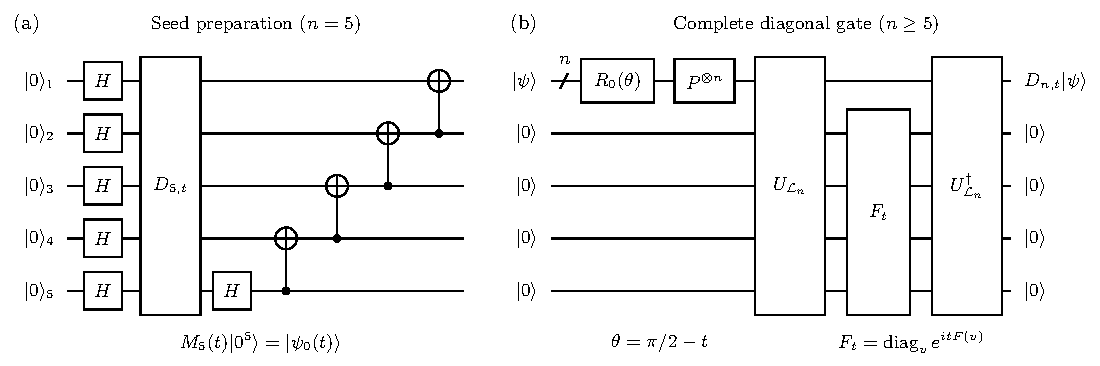
\includegraphics[width=\textwidth]{figures/fig4_clifford.pdf}
  \captionof{figure}{Circuit structure of the measurement unitary. Gates act from left to right.
  (a) Five-qubit seed preparation in the normal form of Ref.~\cite{PauwelsGisin2026}.
  (b) Decomposition of $D_{n,t}$ for every $n\ge5$, with the global phase $-i$ omitted.
  The top wire carries the $n$ data qubits, $P=\operatorname{diag}(1,i)$, and $R_0(\theta)=\exp(i\theta|0^n\rangle\langle0^n|)$ with $\theta=\pi/2-t$.
  $R_0$ is shown as an undecomposed $n$-qubit gate. Its implementation uses one clean ancilla; any of the four auxiliaries, still in $|0\rangle$ at that stage, can serve this role.
  The parity encoding $U_{\mathcal L_n}:|z\rangle|a\rangle\mapsto|z\rangle|a\oplus\mathcal L_nz\rangle$, the four-qubit gate $F_t$, and the inverse encoding implement $e^{itq_n}$ and restore the auxiliaries to $|0\rangle$.
  At $t=0$, $F_t=I$ and the encoding cancels with its inverse; $R_0(\pi/2)$ is the $X$-conjugated multi-controlled $P$ gate, recovering the decomposition of Ref.~\cite{PauwelsGisin2026}.
  At $t=\pi/2$, $R_0=I$.}
  \label{fig:clifford}
\end{minipage}
\par\medskip
\twocolumngrid


附录~\ref{physics:app-hierarchy} 给出完整模四多项式及推导。在文献~\cite{PauwelsLocalization2025,PauwelsGisin2026} 的局域化框架中，这些层级给出所需资源的上界。
